\documentclass[11pt]{article}
\usepackage[letterpaper,margin=.88in]{geometry}
\usepackage{amsmath,amssymb,amsthm,booktabs,tabularx,microtype,hyperref,tikz}
\usetikzlibrary{arrows.meta,positioning}
\hypersetup{colorlinks=true,linkcolor=black,citecolor=black,urlcolor=black}
\newtheorem{theorem}{Theorem}[section]
\newtheorem{proposition}[theorem]{Proposition}
\newtheorem{corollary}[theorem]{Corollary}
\newtheorem{definition}[theorem]{Definition}
\newtheorem{example}[theorem]{Example}
\theoremstyle{remark}\newtheorem{remark}[theorem]{Remark}
\newcommand{\N}{\mathbb N_0}
\newcommand{\cl}{\operatorname{Con}}
\newcommand{\cost}{\operatorname{cost}}
\newcommand{\Rev}{\mathsf{Rev}}
\newcommand{\Ord}{\mathsf{Ord}}
\newcommand{\J}{\mathcal J}
\newcommand{\F}{\mathcal F}
\newcommand{\B}{\mathsf{BANK}}
\newcommand{\W}{\mathsf W}
\newcommand{\V}{\mathsf V}
\setlength{\parindent}{1em}
\title{\textbf{Depths of a Possible Machine}\\[5pt]\large Semi-Ideal Computers, Certified Transformations,\\and the Geometry of Potential Mathematical Intelligence}
\author{Research direction: Brian Tenneson\\Mathematical drafting and analysis: ChatGPT (Picard research protocol)}
\date{24 November 2026 $\mid$ Research edition 001}
\begin{document}
\maketitle
\begin{abstract}
A machine's deductive state does not determine the capabilities of its possible successors. Starting from the semi-ideal computer (SIC), clocked simulation, recoding and formal reflection of \emph{Depths of a Simulation}, we distinguish present competence, attainable capability and discoverable revision. A revision-budgeted settlement profile admits exact finite computation, saturation and optimality certificates. We establish arbitrarily deep revision hierarchies, characterize the attainable shapes of finite potential profiles, and construct a conservative successor whose target-stage performance improves while remaining incomparable under the original clocked simulation preorder. Single-target potential fails to determine joint workload capability. A black-box discovery bound separates inexpensive possible revisions from inexpensive discoveries. A generalized Picard protocol binds preservation, lawful installation and improvement evidence to the parent. The final specialization interprets revisions as sovereign gifts in the 24th century. Established mathematical machinery is credited; the paper is a conditional mathematical study with finite regression checks, not a deployed self-improving machine.
\end{abstract}
\noindent\textbf{Status.} Standalone research companion, not a replacement for the July 27 merged edition or its November 9 audit. All general results are restricted to their stated mathematical hypotheses. No new authority, live agent, or runtime installation is asserted. The term ``24th century'' denotes an underlying sovereign game, not a chronological prediction.
\medskip
\noindent\textbf{Reading map.} Sections 1--3 inherit the SIC foundations and define complete revision-capable configurations. Sections 4--6 develop potential profiles, simulation incomparability, and workload comparisons. Sections 7--9 study discovery, the generalized Picard protocol and sovereign specialization. Sections 10--12 place the results in the literature, report the audit and identify open obligations.
\newpage
\section{Inheritance from the original theory}
The original document \cite{depths} asks what constitutes a computer, how computers can simulate one another, and what a machine can prove about itself. Its Definition 1.2 fixes a formal system $F=(x,y,z)$: alphabet, well-formed finite strings, and finitary partial rules. Its Definition 2.3 fixes a SIC $M=(C,H)$ over $Y\subseteq y$. For $\Gamma\subseteq Y$ and $m\in\mathbb N_+$, $C(\Gamma,m)$ is a subset of $Y$, and $H(\Gamma,m)$ is a bit. The initial state is $C(\Gamma,1)=\Gamma$; formula states grow monotonically; halting persists and freezes the state. A target-search ATP for $\phi$ obeys the sound stopping condition $H=1\Rightarrow\phi\in C$ and eventual halting whenever $\Gamma\vdash_F\phi$. Deductive soundness of its deposits is an additional obligation, for example by rule-driven growth (original Proposition 2.15).

The original Definition 3.15 defines $M\preceq_{\rm clk}N$ by a state injection $f:S_M\to S_N$ and an admissible clock $\rho$ with $\rho(1)=1$, nondecreasing and unbounded, satisfying, for all input states $p$ and all $m$,
\[
 f(C_M(p,m))=C_N(f(p),\rho(m)),\qquad H_M(p,m)=H_N(f(p),\rho(m)).
\]
This is stronger than a comparison of target success or cost. The original Proposition 3.4 makes the set-theoretic state space $S_M=\mathcal P(Y)$; Remark 3.25 explicitly warns that coding every such state is impossible for infinite countable $Y$. We therefore use finite states or specified countable effectively presented configurations whenever claiming an algorithm.

Original Theorem 4.8 transports proofs through invertible recoding and preserves shortest proof length. Definition 4.19 (the Picard Protocol) asks a rule-driven target-search ATP to establish a true assertion that its recoded copy is an ATP, without that target being among its initial hypotheses. Theorem 4.21 exhibits a minimal witness. Part II treats formal self-awareness as a tagged provability structure; Definition 15.17 grades the reflection sequence, and Theorems 20.4 and 21.1 address an idealized mathematician and a reflection-closure machine respectively. Theorem 21.6 distinguishes the competence to establish arbitrarily deep finite reflection from the performance of actually doing so. None of those facts amounts to a claim about consciousness.

Our question is a successor of those questions: what transformations are accessible to a machine, what can it establish about those transformations, and what can it actually accomplish after paying for them? This question does not require a sovereign player in every definition. The authorized-revision interpretation in Section~\ref{sec:sovereign} comes last.

\subsection{An inherited boundary worth repairing}
Original Definition 2.11 uses the non-frozen shortest-proof-layer function for a target-search SIC. If a target first appears at one stage and a different formula first appears later, that definition can violate the freeze-on-halt axiom of Definition 2.3. For example, with $p\to q\to r$ as unary rules, initial $\{p\}$ and target $q$, the shortest proof lengths of $q,r$ are two and three. Freezing the target version at $m_* = \|q\|_F(\Gamma)$ repairs this: set $C(\Gamma,m)=C^{bf}(\Gamma,\min(m,m_*))$, with $\min(m,\infty)=m$. The first-halting-stage identity of Theorem 2.12 survives. This is a local correction proposal to the supplied text, not a claim that its original PDF has been edited. Even a perfectly defined shortest-proof-layer stage is not an executable wall-clock or primitive-operation bound; the 2026 ATLAS amendments already emphasize the distinction between size and search time.

\section{Complete configurations and preservation}
\begin{definition}[Frozen mathematical task]
Fix a formal environment $F$, an authorized context $\Gamma$, a finite target family $\mathcal T$, a sound full-certificate checker $\V$, and a receipt semantics. A receipt for $t\in\mathcal T$ must bind the exact judgment $\Gamma\vdash_F t$, the proof object, its scope and checker identity. The task family and checker remain fixed. Conditional judgments in other contexts cannot silently become unconditional deposits.
\end{definition}
\begin{definition}[Revision-capable configuration]
A configuration is a record $s=(B,K,A,L,u)$ of scoped proof records, operational contract, authority, revision ledger and all other rule-relevant control data $u$ (scheduler phase, obligations, resource constraints, and so on). The observation $B$ may project to the formula set of a SIC; it need not equal the entire state. The set $X$ of complete states carries a directed multigraph with two kinds of labeled transitions: ordinary operations $\Ord$ and committed revisions $\Rev$. Each edge $e$ has a fixed nonnegative cost $w(e)$ and indicator $r(e)=1$ if it is a committed revision, $0$ otherwise. A proposal, verification, refusal or deferral is an ordinary event, not a committed revision. A bundled transaction can instead be one edge only if its total costs and effects are correctly represented.
\end{definition}
Each edge represents an actually legal transition in a specified mathematical model, not a candidate name or an unexplained oracle. Let $G_t\subseteq X$ consist of states containing the required accepted receipt. We do not assume that every state containing the formula $t$ has emitted that receipt. In a portfolio run, individual receipts need not halt the machine; only the declared terminal condition stops it.

\begin{definition}[Certified revision contract]
A revision binds a parent configuration and version; a finite description of the proposed successor and state translation; preconditions, postconditions, authorization and preserved commitments; an increment $\Delta$ of stage-indexed controller theory; exact proof-context transport; a charged cost model; and evidence for those obligations. A fixed external admission checker $\W$ checks the declared claims. The installation event requires a current-parent receipt, a legal authorized decision and execution of the specified transition. A receipt is not installation.
\end{definition}
Separate the controller theory $U_i=U_0\cup\bigcup_{j\le i}\Delta_j$ from the object theory $F$ and its context. The controller ledger records historical versions, not contradictory assertions about one unindexed present. The two checks $\V$ and $\W$ have different subjects. Their soundness is a hypothesis, not a consequence of a machine's self-description.

\begin{theorem}[Conditional inheritance]\label{thm:inherit}
Suppose $U_0$ is consistent and each committed increment carries sound evidence of consistency of $U_{i-1}\cup\Delta_i$ and of the actual operational preservation obligations. Suppose ordinary and revision events preserve the validity and scope of every retained proof record, and every new object receipt is accepted by the unchanged sound $\V$. Then every finite committed prefix has consistent controller theory, every accepted receipt proves its original judgment, and the union of a nested infinite controller chain is consistent in a finitary calculus. No new consequence of $F$ follows merely from revision.
\end{theorem}
\begin{proof}
Induct on committed revisions for controller consistency and on all events for scoped receipt preservation. A contradiction in the union uses finitely many axioms, hence occurs in some finite prefix. The frozen verifier and judgment entail the receipt assertion by soundness. The set of formal consequences is a property of $F,\Gamma$, not the operational graph. This establishes neither termination nor the existence of a finite executable limit.
\end{proof}
This is the inherited consistency-gate principle from the sovereign manual, CDF-C, and the audited basin-escape paper \cite{gift,cdf,basin}. It is used here, not claimed as a new consistency theorem.

\section{Knowledge does not determine capability}
\begin{definition}[Revision-budgeted horizon]
For $s\in X$, $k\in\N$, and $G\subseteq X$, write
\[
 J_k(s,G)=\inf\left\{\sum_{e\in p}w(e):p:s\leadsto G,\ \sum_{e\in p}r(e)\le k\right\},
\]
where the empty path is allowed and the infimum of the empty set is $\infty$. Set $J_\infty(s,G)=\inf_{k\ge0}J_k(s,G)$. For a finite family of target receipts, the potential profile is $\J(s)=(J_k(s,G_t))_{k,t}$. Its budget observation is $\F_{b,k}(s)=\{t:J_k(s,G_t)\le b\}$ in the finite setting where minima are attained.
\end{definition}
This is a cooperative full-information model, not a forced value against an adversary. It is the cheapest legal execution, not the cost of discovering that execution. Costs can count work, elapsed slots, or another predeclared unit but not mix incomparable quantities. In a countably infinite graph, the infimum need not be attained; at an equality boundary use an actual path witness, not merely the infimum.

\begin{proposition}[Knowledge--capability separation]
Even for one fixed formal system, target and sound checker, equal initial formula knowledge and equal deductive closure do not determine $J_0$.
\end{proposition}
\begin{proof}
Use $\Gamma=\{p,p\to q,q\to r\}$ with target $r$. In one operational contract, only individual modus ponens steps are enabled, with unit action cost; receipt emission is bundled into the final step. In the other a certified macro emits an expanded two-step proof in one abstract action. Both preserve the same theoremhood, both have the same initial knowledge, but their minimum action costs are two and one. If a third controller permits only an idle action, its horizon is infinite. The difference is operational access, not a new logical consequence.
\end{proof}
For actual computational cost the expansion and checking cannot be assumed free. This witness deliberately measures actions. A charged macro can cost more than its expanded execution. The original closure abstraction (Theorem 3.30) is not wrong for identifying equal consequence sets; it is simply not a capability-preserving abstraction.

\begin{center}
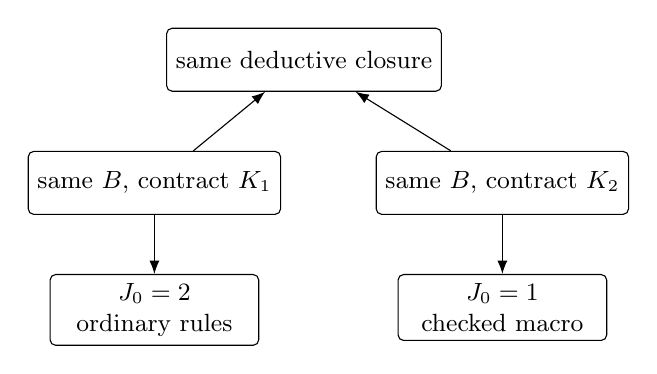
\begin{tikzpicture}[>=Latex, every node/.style={font=\small},b/.style={draw,rounded corners=2pt,minimum width=2.65cm,minimum height=.8cm,align=center}]
\node[b] (a) {same $B$, contract $K_1$};
\node[b,right=1.2cm of a] (b) {same $B$, contract $K_2$};
\node[b,below=.75cm of a] (c) {$J_0=2$\\ordinary rules};
\node[b,below=.75cm of b] (d) {$J_0=1$\\checked macro};
\node[b,above=.75cm of a,xshift=1.9cm] (e) {same deductive closure};
\draw[->] (a)--(c);\draw[->](b)--(d);\draw[->](a)--(e);\draw[->](b)--(e);
\end{tikzpicture}

\small Figure 1. Deductive closure forgets operational distinctions that determine a settlement horizon.
\end{center}

\section{The geometry of potential development}
\begin{theorem}[Layered potential and finite saturation]\label{thm:layers}
Let $X$ be finite, $|X|=n\ge1$, with a complete finite edge list and nonnegative rational costs. Then:
\begin{enumerate}
\item $J_{k+1}(s,G)\le J_k(s,G)$ for every $k$;
\item $J_k$ equals ordinary shortest-path cost in the graph of states $(x,i)$, $0\le i\le k$, with edges $(x,i)\to(y,i+r(e))$ whenever $e:x\to y$ and the endpoint index is at most $k$, starting at $(s,0)$ and targeting $G\times\{0,\ldots,k\}$;
\item $J_\infty=J_{n-1}$, and every finite $J_k$ has a witnessing path of at most $n-1$ edges.
\end{enumerate}
\end{theorem}
\begin{proof}
Increasing $k$ only enlarges the path set. Each legal path of revision count at most $k$ lifts uniquely from $(s,0)$ by summing revision indicators; projecting a layered path yields the corresponding legal path with equal charge. For the last assertion, delete any closed segment between repeated complete states of a finite path. Nonnegative cost and nonnegative revision count ensure neither resource increases. Legal continuation is preserved because the repeated state includes all relevant history, authority and budget information. A simple path remains, with at most $n-1$ edges. There are finitely many such paths in a finite multigraph. A finite infimum is therefore attained and no revision count above $n-1$ improves it.
\end{proof}
\noindent\textbf{Algorithm.} Build the layered graph and run a nonnegative shortest-path algorithm (e.g. Dijkstra \cite{dijkstra}). There are $(k+1)n$ vertices and at most $(k+1)|E|$ edges, with $k$ capped at $n-1$ by the theorem. A binary-heap implementation costs $O((k+1)(n+|E|)\log((k+1)n))$ arithmetic/queue operations under the usual indexed-heap implementation; exact rational arithmetic and input construction costs are additional. The finite graph itself may be exponentially large or impossible to enumerate in an unrestricted ATP. No complexity claim is made about synthesizing this graph.

\begin{theorem}[Strict revision-depth hierarchy]\label{thm:depth}
For every positive integer $d$ there exists a finite revision-capable configuration with one fixed sound proof task and unchanged object-theory deductive closure such that
\[
 J_0=J_1=\cdots=J_{d-1}=\infty,\qquad J_d=d+1.
\]
\end{theorem}
\begin{proof}
Fix the true hypothesis $p$ and a valid unary formal inference $p\Rightarrow t$ (e.g. $t=p\lor p$). The controller has states $s_0,\ldots,s_d$, each carrying $p$ and the same proof theory. The only non-idle transitions before $s_d$ are the successive authorized revisions $s_i\to s_{i+1}$, each unit cost, with distinct version-indexed controller facts. At $s_d$ an ordinary proof-and-receipt action of cost one becomes enabled and leads to $g$. No earlier state has that action. A finite controller table with disjoint version-indexed facts is a model of its stipulated controller specification. Each legal route to $g$ crosses every revision edge, so at least $d$ revisions and one ordinary action are necessary. The chain itself attains that charge. All object consequences remain unchanged. This establishes a family of abstract finite controller models, not the admissibility of every chain in a particular gift catalogue.
\end{proof}
\begin{center}
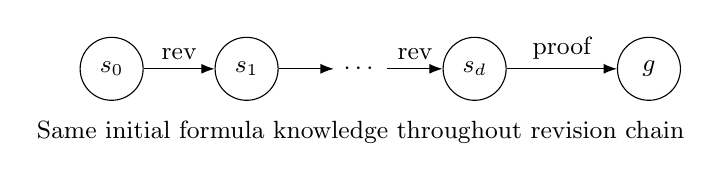
\begin{tikzpicture}[>=Latex, every node/.style={font=\small},v/.style={draw,circle,minimum size=.8cm}]
\node[v](a){$s_0$};\node[v,right=.9cm of a](b){$s_1$};\node[right=.7cm of b](c){$\cdots$};\node[v,right=.7cm of c](d){$s_d$};\node[v,right=1.4cm of d](g){$g$};
\draw[->](a)--node[above]{rev}(b);\draw[->](b)--(c);\draw[->](c)--node[above]{rev}(d);\draw[->](d)--node[above]{proof}(g);
\node[below=.35cm of c]{Same initial formula knowledge throughout revision chain};
\end{tikzpicture}

\small Figure 2. No fixed finite revision horizon captures all possible machines.
\end{center}
The word ``depth'' has three different meanings here: original proof length, original reflection rank, and the number of legally committed revisions required to enable a settlement. Theorem~\ref{thm:depth} separates the third from the first two. It does not say that acquiring higher depth is desirable.

\begin{theorem}[Realization of finite potential profiles]\label{thm:realize}
Fix an integer $d\ge0$ and a finite nonempty target set $\mathcal T$. For each $t$ let $v_{0,t},\ldots,v_{d,t}$ be a nonincreasing sequence in $\mathbb Q_{\ge0}\cup\{\infty\}$. There is a finite revision-capable model with initial configuration $s_0$ and these exact singleton profiles:
\[
 J_k(s_0,G_t)=v_{\min(k,d),t}\qquad(k\in\N,\ t\in\mathcal T).
\]
The initial formula knowledge and deductive closure can be identical at all nonterminal revision states. If $v_{j,t}\ge j\eta$ whenever finite, for a fixed rational $\eta\ge0$, the construction can give every revision edge cost $\eta$.
\end{theorem}
\begin{proof}
Use a common fixed true seed and distinct target consequences with valid finite proof packets, and a chain $s_0\to\cdots\to s_d$ of revision edges each of cost $\eta$. Choose $\eta=0$ if no positive charge satisfies the stated condition. At each $s_j$ add a terminating ordinary proof-and-receipt edge for $t$ exactly when $v_{j,t}$ is finite, of cost $v_{j,t}-j\eta$. Give the endpoint only the receipt for that target; there are no outgoing edges from terminal endpoints. All costs are nonnegative. Every successful path for $t$ uses a chain prefix of length $j\le\min(k,d)$ followed by the designated edge, with total charge $v_{j,t}$. The minimum of these values is precisely $v_{\min(k,d),t}$, including the all-infinite case. The revision states can share the same seed and fixed formal calculus, differing only in versioned authorization tables. These finite tables can be interpreted literally in the controller model.
\end{proof}
This characterization is an abstract expressiveness statement, not a proposal to declare real computations costless. A positive cost floor imposes additional resource restrictions; actual checker and proof-output cost must be charged. Within the unconstrained nonnegative-cost finite model, monotonicity and eventual constancy are the only restrictions on the shape of an individual potential profile. The theorem realizes profiles separately for each target, not joint workloads; Section 6 explains why this matters.

\subsection{Certificates rather than merely computed scores}
\begin{theorem}[Potential certificates]\label{thm:cert}
In the finite layered graph, a function $h$ with nonnegative extended rational values, $h=0$ at all goal nodes, and
\[
 h(v)\le w(v,u)+h(u)\quad\text{for every edge }v\to u
\]
certifies a lower bound on remaining shortest-path charge. A legal path with charge $h(v)<\infty$ certifies equality. A set $D$ containing the start, disjoint from the goals, and closed under all outgoing layered edges certifies impossibility. Each finite instance admits an exact certificate of optimality or impossibility.
\end{theorem}
\begin{proof}
Iterate the displayed inequality along any finite goal path. Its last value is zero, so $h(v)$ is at most the path charge. A matching path gives equality. If $D$ is closed, induction on path length shows no path from $D$ reaches a goal. For existence of certificates, let $h$ be actual shortest-path distance to the goals, using $\infty$ for unreachable nodes; its inequalities follow by concatenation. A finite distance is attained by Theorem~\ref{thm:layers} applied to the layered graph, or by ordinary cycle deletion. The non-reaching nodes form a closed set. All comparisons are local checks on an explicitly complete finite graph.
\end{proof}
This is the standard shortest-path potential principle in a revision-budgeted state space; it connects directly to \emph{Where Infinity Breaks} and the proof-cut work \cite{infty,obstruction}. A lower bound on a restricted candidate graph is not necessarily a lower bound on the full graph. An externally checked abstraction must relax every relevant concrete transition at no greater cost and preserve goal observations in the appropriate direction. Without that coverage, a negative conclusion is restricted to the supplied graph.

\section{Revision reachability is not simulation}
Define $s\preceq_{\rm rev}t$ when a finite legal path using only revision edges leads from $s$ to $t$; include the empty path. If proposal/administrative events are required, use complete authorized revision transactions as edges or define a separately named mixed reachability relation. With states that include full history, reachability is reflexive and transitive by concatenation; its mutual-reachability equivalence yields the usual partial order on strongly connected classes. If each commit strictly extends an immutable ledger, there are no nonempty revision cycles, and the relation is already antisymmetric on complete configurations. A rollback of active policy need not return to the old complete state. Forgetting the ledger can create apparent cycles.

Define $s\preceq_{\rm pot}t$ when $J_k(t,G_a)\le J_k(s,G_a)$ for every specified $a,k$ in a common observation contract. This is a preorder by numerical transitivity. Neither relation forces the other: an authorized change may cost more or remove useful actions; two machines with equal or ordered potential need not be linked by a permitted revision. They also need not admit a clocked simulation, as the next construction proves.

\subsection{A conservative faster successor incomparable under clocked simulation}
\begin{theorem}[Clocked incomparability with strict target-stage improvement]\label{thm:incomp}
There are two finite, sound target-search SICs $M,N$ for the same base formal theory and target such that $N$ halts no later than $M$ on every input and strictly earlier on one, but neither $M\preceq_{\rm clk}N$ nor $N\preceq_{\rm clk}M$ in the original Definition 3.15. The successor's shortcut is deductively conservative.
\end{theorem}
\begin{proof}
Let $Y=\{p,q,r\}$ with unary rules $p\Rightarrow q$ and $q\Rightarrow r$, and target $r$. Treat the formulas as strings and the rules as the stipulated formal system. If desired, interpret $q=p\lor p$ and $r=q\lor q$ in a sound propositional calculus. At stage one both machines expose the input $A\subseteq Y$. If $r\in A$, halt and freeze. Otherwise $M$ adjoins $r$ if $q\in A$, adjoins $q$ if $p\in A$ but $q\notin A$, and does nothing otherwise. Repeat until halt. $N$ adjoins $r$ whenever $p$ or $q$ is present, using the certified derived rule $p\Rightarrow r$ when necessary; it exposes the final conclusion, not the macro's intermediate $q$. The expanded proof remains available as provenance. Both are monotone in stage, freeze on halt, and are target-search ATPs on all eight inputs. $N$ is rule-driven in the conservative extended presentation, not claimed rule-driven for the original primitive rule list.

For input $\{p\}$, $M$ has three distinct states $\{p\},\{p,q\},\{p,q,r\}$; every trajectory of $N$ has at most two. An injective state map makes simulation of $M$ into $N$ impossible, regardless of admissible clock.

In the other direction both state spaces equal $\mathcal P(Y)$, so the injection is a bijection. It preserves initial halting, and because the clock is unbounded it preserves eventual halting in both directions. Hence it maps the three initially nonhalting but eventually halting inputs $\{p\},\{q\},\{p,q\}$ bijectively onto themselves. The three inputs of $N$ end at three distinct terminal states, whereas those of $M$ end at only two distinct terminal states. Taking a sufficiently late common stage contradicts injection. Finally, halting stages are 3 versus 2 on $\{p\}$; both are 2 on $\{q\},\{p,q\}$, both 1 on any input already containing $r$, and both infinite on the empty input. The derived rule expands to two legal primitive steps; it adds no theoremhood.
\end{proof}
\begin{center}
\begin{tabular}{ccll}
\toprule Input & $M$ stage / $N$ stage & $M$ terminal state & $N$ terminal state\\\midrule
$\{p\}$ & $3/2$ & $\{p,q,r\}$ & $\{p,r\}$\\
$\{q\}$ & $2/2$ & $\{q,r\}$ & $\{q,r\}$\\
$\{p,q\}$ & $2/2$ & $\{p,q,r\}$ & $\{p,q,r\}$\\\bottomrule
\end{tabular}
\end{center}
The comparison is deliberately at the original SIC exposed-formula state and halting-stage level. It does not show that an implementation with full internal macro states cannot simulate $M$, nor that a one-stage macro saves primitive work. A revision granting this macro could preserve the old policy as an optional alternative in its complete controller. The two fixed-policy SIC snapshots would still have the incomparability just proved. This is a concrete reason not to use the clocked preorder alone as the improvement criterion.

\section{Potential is richer than a scalar intelligence score}
\begin{theorem}[Single-target potential is not portfolio potential]\label{thm:portfolio}
There are two finite legal configurations having identical initial knowledge and identical $J_k$ for every singleton target and every revision budget, but different cost to achieve both targets in one continuing execution.
\end{theorem}
\begin{proof}
Let $a,b$ be two consequences of a common fixed seed, and let their receipts persist once issued. In system $X$, the controller may issue $a$ or $b$ at unit cost, but an irreversible authorization choice prevents issuing the other. In system $Y$, either may be issued at unit cost and then the other at unit cost. Use no revision edges. Both have singleton horizons one for each target, independent of $k$. For the joint goal requiring both receipts, the horizons are respectively $\infty$ and two. Both systems can be represented by finite explicit controller tables and a fixed sound checker for the two proof packets.
\end{proof}
Consequently we must distinguish a profile indexed by targets from a profile indexed by workloads, joint receipt goals, or adaptive sequences of queries. This is relevant to an ATP whose investment in a lemma or macro pays off across many targets. A vector of optimal costs for separate runs does not certify that one strategy achieves all its coordinates simultaneously.

\begin{definition}[Portfolio-aware potential]
For a declared workload family $\mathcal U$ of terminal receipt predicates on complete states, replace $G_t$ by every $G_U$, $U\in\mathcal U$, in $\J$. The componentwise order is an exact comparison of the corresponding \emph{individual optimum values}, not a guarantee that one common policy attains them all. An ordered workload may be encoded by a task-progress coordinate in the complete state.
\end{definition}
\begin{proposition}[Costed continuation transport]\label{thm:transport}
Suppose a map $f:X\to X'$ preserves goal membership in the forward direction for each declared goal, and each source edge can be implemented by a finite legal path from $f(x)$ to $f(y)$ costing at most $w(e)$ and using at most $r(e)$ revisions. These paths must be executable in the image of each complete endpoint, not just in a matching projection. Then $J'_k(f(s),G'_U)\le J_k(s,G_U)$ for all $k,U$.
\end{proposition}
\begin{proof}
Transport each finite source path by concatenating the edge implementations. The endpoint is a goal by the observation condition, and both resources are bounded by the original sums. Taking infima proves the result, including unreachable source goals. Empty source paths use the goal condition directly.
\end{proof}
The hypothesis is a sufficient weighted forward refinement, not a necessary condition for numerical dominance. If a setup transition to $f(s)$ costs $K$ and uses $h$ revisions, the corresponding bound from its source is $K+J_k(s,G_U)$ with revision budget $h+k$, provided the target path remains legal after setup. Composition of transport maps follows by path concatenation; setup costs add only when measured on actual compatible successive states. This builds on the existing successor and revision quotient literature \cite{successor,quotients,alur}. It makes explicit why no comparison of abstract capabilities alone implies economically favorable self-modification.

\section{Discoverability: from possible machine to found machine}
The original Picard competence--performance distinction now has an operational analogue. We distinguish:
\begin{enumerate}
\item a semantically admissible transformation (the external conditions are true);
\item a certifiably admissible transformation (an accepted finite witness exists);
\item a discovered transformation (a particular process has actually produced its accepted witness);
\item an installed and exercised transformation (the authorized legal events actually occur).
\end{enumerate}
If the external gate is sound, (2) implies (1). If discovery and installation obey the contract, (4) implies (3) implies (2) for that history. The converses are not automatic. A semantic graph is not generally executable. One may compare separate graphs using the same costs on common edges; for a sound restricted graph its optimum cannot beat the semantic optimum, assuming the same initial state and goal observations. If the semantic graph's costs omit certificate discovery, it is only an ideal comparator, not the real charged value.

\begin{theorem}[Effective certificate discovery, not effective omniscience]
Suppose at each finitely described parent, candidate revision--certificate pairs are effectively enumerable, checks terminate, and accepted pairs yield effectively computable legal successor descriptions (when authorization and execution are included). Assume the analogous effective interfaces for ordinary transitions and goal recognition. Then existence of a finite certified route to an accepted goal is recursively enumerable. With a computable exhaustive finite successor list and known depth bound, existence is decidable. The latter claim extends to a bounded rational cost test if all edge costs are computable exact rationals.
\end{theorem}
\begin{proof}
Dovetail enumeration of finite path descriptions and their finite checks, including parent matching and execution permissions. Any genuine finite route is eventually enumerated and checked; accept only a successful route. With finite complete successor lists and bounded depth, exhaustive traversal terminates. Exact rational addition and comparison decide the cost condition. Neither construction implies that traversal and replay together fit the same cost bound; that needs separate accounting.
\end{proof}
\begin{proposition}[A semantic barrier]
Suppose the permitted contract language uniformly includes a candidate $g_e$ with otherwise admissible finite operational effect and cumulative arithmetic increment $\varphi_e$ asserting that machine $e$ never halts. Assume the consistent arithmetic baseline contains PA, has a standard model compatible with the operational facts, and the other admissibility obligations are independent of $e$. Then semantic admissibility of $g_e$ is equivalent to nonhalting. There is no sound effective certificate gate that is complete for this family.
\end{proposition}
\begin{proof}
If $e$ does not halt, the compatible standard model satisfies $\varphi_e$. If it halts, a finite computation proves its halting in PA, so adjoining $\varphi_e$ is inconsistent. A sound complete effective finite-witness gate would enumerate precisely the nonhalting indices by dovetailing all witnesses, which is impossible. The conclusion is conditional on this contract-language expressivity; it is not a claim about the admissibility of any particular historical atom in GBG+S.
\end{proof}
This is an adaptation of standard halting/co-halting barriers and the author's consistency-frontier research, not a new undecidability result about arbitrary machines. A failed bounded search must be reported as unresolved, not as proof of impossibility.

\subsection{An exact discovery overhead in a restricted information model}
\begin{theorem}[Hidden revision query lower bound]\label{thm:query}
Consider $n\ge1$ candidates with one hidden eligible index $i$. The only information interface is a unit-cost query returning whether a specified candidate is eligible. An accepted positive query is required for installation; no other observation identifies $i$. Every eligible candidate has the same installation and subsequent proof charge $a\ge0$. Then the best worst-case guaranteed total charge for deterministic discovery and execution is $n+a$. Under the uniform hidden-index distribution, the best expected total charge for any always-correct randomized or deterministic strategy is $(n+1)/2+a$.
\end{theorem}
\begin{proof}
Before a positive answer, all responses are negative. The sequence of distinct indices tried on this transcript must eventually cover all indices, because each omitted index is a possible hidden state. Repeating a query does not help. A deterministic strategy faces the index appearing last, requiring $n$ queries, and a permutation scan attains the bound. Under a uniform index, for each fixed random seed of a correct strategy the first positive query has rank at least the position in its order of first occurrences. The average of positions is $(n+1)/2$; averaging over random seeds preserves the lower bound. Scanning a fixed permutation attains it. Add the common execution charge $a$.
\end{proof}
With a supplied correct index, one positive query and execution cost $1+a$ suffice. Thus the gap between knowing an admissible gift and having to discover it is arbitrarily large even with a finite candidate domain and constant per-candidate test cost. This elementary black-box bound does not assert that real mathematical descriptions conceal their useful structure; they may expose exploitable invariants. In particular it does not contradict receipt-guided revision selection in \cite{receipts}. It motivates searching for structural information that replaces black-box queries, and charging the cost of acquiring that information.

\section{A generalized Picard protocol}
The original Picard Protocol certifies a recoded version of a machine. A stronger operational task is to construct a nontrivially revised machine and certify an advantage while preserving the mathematical contract. There is no need to claim that a machine proves its own unrestricted consistency. Instead the protocol uses a parent-bound certificate with explicit external assumptions.
\begin{definition}[Successor Picard packet]
For a fixed parent $s$, workload $\mathcal U$, and accounting convention, a packet contains:
\begin{enumerate}
\item a finite successor description $s'$ and a legal state-transfer implementation;
\item a proof of scoped object-certificate preservation and a controller consistency witness satisfying Theorem~\ref{thm:inherit};
\item a proof that the intended successor is a sound ATP for its declared target domain, including completeness where promised; for an unbounded fair search this requires effective coverage, acceptance-complete checking and actual fair service;
\item a separate certified comparison with a predeclared baseline under the same task, receipt semantics and accounting, including charged discovery, checking, installation, execution and recovery where required;
\item an externally accepted parent-bound receipt, followed by a distinct authorized installation event and a recorded outcome if exercised.
\end{enumerate}
A proposal packet that proves only items 1--3 is a certified candidate, not yet a demonstrated improvement. An example that proves a route exists need not prove that the particular discovery policy finds it. No part of the definition requires an autonomous installation.
\end{definition}
\begin{theorem}[Finite charged improvement criterion]\label{thm:cost}
Let $L$ be a verified lower bound on the baseline's total charge for a specified workload, under its declared contract. If a legally executable discovery--installation--settlement trace for a successor has certified upper charge $U<L$, with identical required receipts, then its trace is strictly cheaper than every baseline trace covered by $L$. If only a baseline measured or designated trace of charge $L$ is given, the strict comparison is only with that trace. A successor that admits the old strategy but incurs mandatory additional cost has no automatic net advantage.
\end{theorem}
\begin{proof}
The fully charged successor trace costs at most $U$. Every baseline trace covered by the lower bound costs at least $L$, so strict inequality gives the claim. The designated-trace version follows from the same numerical comparison. Optionality of a strategy does not remove costs required to make that strategy executable.
\end{proof}
For repeated independent matched tasks, if baseline cost is $a$, revised per-task cost is $b$ and one-time discovery/adoption cost is $K$, net improvement over $m$ repetitions occurs exactly when $m(a-b)>K$, assuming no other cost differences. This is the established amortization comparison used in CDF-C and the successor work, not a new speedup theorem. It is essential to freeze caching, initial knowledge and workload. An actual theorem prover is not improved merely because a research paper declares it improved.

\subsection{From existential paths to guaranteed play}
If a state has adversarially or nondeterministically selected outcomes, replace the directed graph by actions with nonempty finite outcome sets, each outcome carrying its cost. In a finite ranked complete game whose rank strictly decreases on every nonterminal move, let $V(x,k)$ be the least worst-case charge for settling with at most $k$ commits on every branch. At goal states set $V=0$; at other terminals set $V=\infty$. For legal actions with revision indicator $r(a)$,
\[
 V(x,k)=\min_{a:r(a)\le k}\max_{(y,w)\in\mathrm{Out}(x,a)}\{w+V(y,k-r(a))\}.
\]
A minimum over no actions is infinity. Backward induction on rank establishes the recurrence by the first-action decomposition. A selected minimizing action at every reachable decision boundary supplies a winning policy if the value is finite. For a certified upper bound every possible continuation of that policy must be covered; for a losing-set witness every allowed action must have at least one permitted successor in the losing region of the budget-expanded game. This is the ranked game construction of \cite{infty} with an extra revision-count coordinate. It is not valid to replace the maximum with a favorable single successor or to apply the acyclic recurrence without addressing cycles, nontermination and fairness. Hidden states require belief-state strategies rather than access to their true values.

\section{The 24th-century specialization}\label{sec:sovereign}
In the author's terminology a 24th-century machine operates in an underlying sovereign game. The sovereign rules determine which gifts can be admitted and exercised. The results above require only a legal complete-state transition model. Thus the specialization is to make the controller's revision edges correspond to admitted and actually exercised gifts, retaining the exact object-theory proof task. The stage-indexed controller consistency proof is not a substitute for an interpretation of all gifts in GBG+S.

The audited sovereign manual \cite{gift} supplies a typed, cumulative admission discipline and a restricted structural existence construction; it does not establish unrestricted syntactic relative consistency. For a faithful implementation, a candidate's support-indexed grammar, current parent, cumulative increments, observable novelty, identity and authorization, STOP status, activation, and actual legal player move must satisfy that rulebook. The abstract depth-$d$ chains of Theorem~\ref{thm:depth} must not be called actual GBG+S witnesses until all those obligations have been discharged. The count $k$ in this paper counts commits, not the number of atom names; repeated atoms inside a gift do not change its distinct-support count. A finite vocabulary does not automatically give an effectively exhaustive finite expression catalogue. CDF-C has its own independent contract and clock/credit restrictions. A legal permission never implies compulsory installation.

\begin{center}
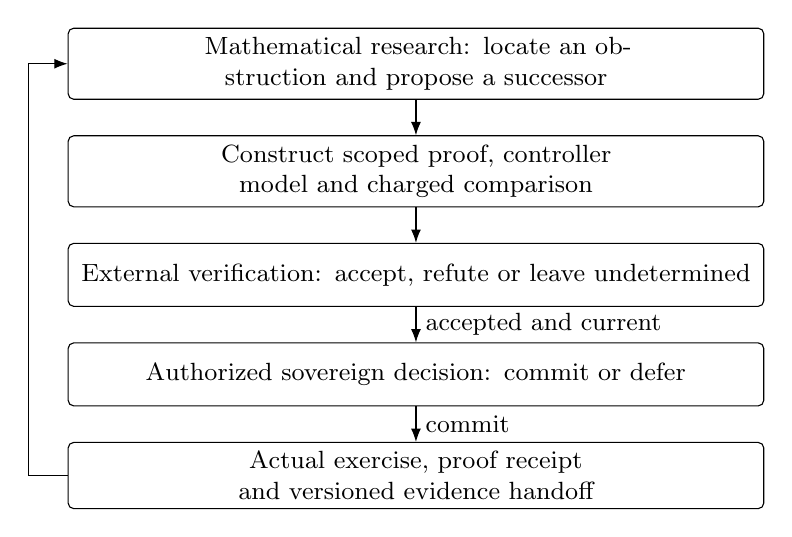
\begin{tikzpicture}[>=Latex, node distance=.45cm, every node/.style={font=\small},b/.style={draw,rounded corners=2pt,text width=8.6cm,minimum height=.8cm,align=center}]
\node[b](a){Mathematical research: locate an obstruction and propose a successor};
\node[b,below=of a](b){Construct scoped proof, controller model and charged comparison};
\node[b,below=of b](c){External verification: accept, refute or leave undetermined};
\node[b,below=of c](d){Authorized sovereign decision: commit or defer};
\node[b,below=of d](e){Actual exercise, proof receipt and versioned evidence handoff};
\draw[->](a)--(b);\draw[->](b)--(c);\draw[->](c)--node[right]{accepted and current}(d);\draw[->](d)--node[right]{commit}(e);
\draw[->] (e.west) -- ++(-.5,0) |- (a.west);
\end{tikzpicture}

\small Figure 3. A proposed research cycle; the loop is not an executable installation.
\end{center}
\noindent\textbf{Illustrative application.} An obstruction certificate in an original frozen proof controller may certify an infinite operational horizon. A guarded relinquishment of a veto can enable an already valid ordinary proof, as in Basin Escape v0.3 \cite{basin}. The profile $J_0=\infty,J_1<\infty$ then has operational meaning for that constructed witness. An obstruction in the logical theory itself cannot be eliminated merely by a conservative operational gift. A newly admitted edge invalidating one old losing certificate is not sufficient to prove settlement. The revised controller needs a new positive proof or a branch-complete winning certificate. This is the connection between the potential geometry here and obstruction-directed MAPQUEST \cite{obstruction}.

\section{Relationship to prior research and novelty boundaries}
The paper deliberately avoids attributing established mathematical machinery to a new machine. The following are the nearest identified dependencies, not an exhaustive systematic review of all literature.
\begin{center}\small
\begin{tabularx}{\textwidth}{@{}>{\raggedright\arraybackslash}p{.29\textwidth}X@{}}
\toprule Prior research & Relationship and limit of present contribution\\\midrule
Cook--Reckhow (1979) \cite{cook} & Proof-system comparison concerns lengths/sizes and efficient translation; our fixed-policy stage comparison is a different observable. Neither gives automatic proof-discovery speedup.\\
Schmidhuber's G\"odel machines \cite{godel} & Prior self-referential proof-guided improvement. Here an externally gated contract and distinct revision-depth profile replace any claim of globally optimal internal rewriting.\\
Necula (1997); Hicks--Nettles (2005) \cite{necula,hicks} & Proof-carrying code and dynamic updating precede our packet idea. The application here tracks exact mathematical receipts and possible successor capability.\\
Alur et al. (1998) \cite{alur} & Alternating refinement precedes branch-sensitive strategy transport; our cooperative comparison is weaker and explicitly scoped.\\
Paige--Tarjan (1987); Dean--Givan (1997) \cite{paige,dean} & Partition refinement and behavioral abstractions are established. We do not claim an original general quotient algorithm.\\
Sutton--Precup--Singh (1999) \cite{options} & Temporally extended actions precede the certified macro example. Our costs and verifier semantics are specialized to proof tasks.\\
Author's W1--W3, successor and CDF-C papers \cite{costgame,quotients,receipts,successor,cdf} & Costed revision, future-sufficient quotients, receipt-guided selection, lineage and gated improvement already exist in this research program. This paper organizes their relationship to the original SIC clocked preorder and develops the explicit separation, revision-depth and portfolio examples.\\\bottomrule
\end{tabularx}
\end{center}
Theorem~\ref{thm:incomp} is a particularly targeted extension of the original SIC theory: it preserves that theory's exact state-map and clock quantifiers, rather than replacing them with a different simulation relation. Theorems~\ref{thm:layers} and \ref{thm:cert} are applications of standard resource expansion and shortest-path mathematics. The strict-depth and portfolio constructions are concrete separations for the proposed model. The profile realization theorem characterizes the possible finite-horizon curves in that abstract model; it does not characterize realizable hardware or sovereign atom catalogues. Their historical priority is not established. The hidden-query result is an elementary information-interface lower bound; it should not be presented as a novel general search lower bound.

\section{Computational checks and proof audit}
A separate standard-library Python script \texttt{depths\_possible\_checks.py} accompanies this edition. It uses a fixed seed (20261124) and performs two independently structured finite path calculations: layered Dijkstra and exhaustive simple-path enumeration. Graphs include zero-charge edges, unreachable vertices and cycles. A separate exhaustive finite-state check tests the clocked incomparability witness; both SICs are constant after stage three, so the clock search needs only the truncated values at stages two and three and an unbounded extension. Initial halting partitions restrict the bijections to $4!4!$ possibilities per direction; all six nondecreasing pairs of truncated stage values are checked. A further randomized finite check constructs the profile-realization models, including positive revision costs and infinite entries, and compares every tested target and budget with its prescribed value. The numerical output is:
\begin{center}
\begin{tabular}{lr}
\toprule Executed check & Count\\\midrule
Generated finite directed graphs & 240\\
Layered versus simple-path scalar comparisons & 29,429\\
Monotonicity comparisons & 29,429\\
Saturation comparisons & 8,502\\
Clock-map and clock-prefix combinations, both directions & 6,912\\
Strict depth chain examples & 30\\
Profile realization comparisons & 1,929\\\bottomrule
\end{tabular}
\end{center}
All assertions passed. These counts are regression checks, not independent proof-assistant certificates and not evidence of ATP speedup. They do not test unrestricted gift admissibility, full proof verification, arithmetic consistency, or actual runtime migration.

\subsection{Revision register}
\begin{center}\small
\begin{tabularx}{\textwidth}{@{}p{.30\textwidth}X@{}}
\toprule Potential overclaim or defect & Controlling repair in this edition\\\midrule
SIC target halts yet continues growing & Section 1 freezes the shortest-layer target-search version; retains original source separately.\\
Equal knowledge implies equal future & Section 3 requires full state; macro action count is not runtime.\\
Unbounded potential always attained & Theorem~\ref{thm:layers} restricts attainment and finite saturation to complete finite graphs and nonnegative resources.\\
Cycle deletion may discard history & Only delete repetitions of complete states, never repetitions of projected knowledge.\\
Faster successor must simulate predecessor & Theorem~\ref{thm:incomp} treats all eight initial states, injectivity, halting and unbounded clock, with explicit macro provenance distinction.\\
Separate optimal targets imply joint optimum & Theorem~\ref{thm:portfolio} exhibits irreversible choices and distinct joint goal semantics.\\
Potential equals discoverability & Section 7 distinguishes semantic, certified, found and installed transformations; query bound has an explicit information model.\\
Admission equals exercise & Sections 2, 8, 9 bind the current parent and separate checking from authorized commit.\\
One path implies guaranteed settlement & Section 8 states the ranked all-outcomes recurrence and its limits.\\
Sovereignty proves every revision legal & Section 9 restricts transfers to checked contracts; no unrestricted GBG+S consistency claim.\\\bottomrule
\end{tabularx}
\end{center}

\section{Open problems and conclusion}
\textbf{Future-sufficient potential.} Characterize the weakest effectively checkable equivalence on complete machine states that preserves a specified family of future revision-budgeted workload values and admits legal lifting of actions. Equality of singleton values is insufficient. Strong behavioral refinements are sufficient but may be much finer than needed. Compare with W2's existing stronger structural quotient, rather than rediscovering it.

\textbf{Obstruction-guided discovery.} Given a certified bound on settlement in the current controller, find a nontrivial family where structural obstruction information yields a provably cheaper search for admissible revisions than an equal-information baseline. The black-box query bound identifies a regime in which merely possessing a candidate grammar is not enough. The aim is a theorem or a controlled experiment about finding useful revisions, not a known gift inserted by hand.

\textbf{Successor incomparability and strength.} Extend Theorem~\ref{thm:incomp} to costed, fully charged implementations or explicit proof-size families, with independently justified lower bounds. Study when a better workload profile admits an efficient simulation in a richer state space, and when it cannot. The existing result is finite and stage-based, not asymptotic.

\textbf{Discoverable depth.} Study families where the cheapest semantic route, cheapest finitely certified route, and cheapest route achievable by a fixed discovery process are different. Establish the appropriate effective representation and information model before claiming a gap. The present arithmetic barrier depends on contract expressivity, and the finite query theorem depends on hidden-index access.

\textbf{Practical next experiment.} Freeze an ATP calculus, a held-out target workload and a baseline search policy. Compare (i) frozen search, (ii) fixed catalogue of conservative checked macros, (iii) obstruction-guided proposal and external revision admission. Charge failed proposals, certificate construction and validation, migration, proof expansion, search and recovery. Record full receipt success, uncertainty and costs; do not infer empirical benefit from the abstract witness. No such deployment was performed in preparing this paper.

The original \emph{Depths of a Simulation} defined machines and compared their computational behaviors. The present companion adds a geometry of possible operational futures. Its principal distinction is between what a machine can prove, what it could become, and what it can actually discover and lawfully become. The external certificate boundary remains the same even as the operational possibilities change.

\noindent\textbf{AI and verification disclosure.} Mathematical drafting, literature triage, proofs, analytical revisions and finite Python checks were performed with ChatGPT in the Picard research protocol under the stated human research direction. The literature review is targeted, not exhaustive. The author-supplied source is preserved. No independent proof assistant checked the general theorems; no empirical ATP benchmark, autonomous successor, publication, or architecture upgrade was carried out. All adoption and further dissemination remain separate decisions.

\begin{thebibliography}{99}\small
\setlength{\itemsep}{0pt}\setlength{\parsep}{0pt}
\bibitem{depths} B. Tenneson, \emph{Depths of a Simulation and Formalized Self-Awareness}, merged edition 1, 27 July 2026; ATLAS v2 correction, 9 Nov. 2026. Supplied 102-page edition, especially Defs. 2.3, 3.15, 4.19 and Thms. 3.30, 4.8, 4.21, 20.4, 21.1, 21.6.
\bibitem{gift} B. Tenneson (research direction), \emph{From the Boring Game to the Last Gift}, selective braid v4v3, 23 Nov. 2026. Restricted sovereign-gift structural construction and cumulative admission.
\bibitem{cdf} B. Tenneson, with ChatGPT, \emph{CDF: Certified Discovery Federation}, v13, 23 Nov. 2026, Section 21.
\bibitem{basin} B. Tenneson (research direction), ChatGPT (Picard protocol), \emph{Basin Escape: Sufficient Conditions, Guarantees, and Limits}, v0.3, 24 Nov. 2026.
\bibitem{infty} B. Tenneson (research direction), \emph{Where Infinity Breaks: Certificates of Impossibility, Optimality, and Model Repair}, Settlement Calculator supporting documentation, supplied 24-page edition.
\bibitem{obstruction} B. Tenneson (research direction), ChatGPT (Picard protocol), \emph{The Geometry of Mathematical Obstruction}, research edition 001, 24 Nov. 2026.
\bibitem{successor} B. Tenneson (research direction), DATA MIND / ChatGPT, \emph{The Discoverer and Its Successor}, audited v2, 16 Nov. 2026.
\bibitem{costgame} B. Tenneson (research program), \emph{Certified Revision as a Costed Mathematical Game (W1)}, \href{https://btenneson.github.io/Mathematics-of-certifiable-self-improvement/}{research library}.
\bibitem{quotients} B. Tenneson (research program), \emph{Future-Sufficient Revision Quotients (W2)}, same research library.
\bibitem{receipts} B. Tenneson (research program), \emph{The Price of Knowing Which Revision to Make (W3)}, same research library.
\bibitem{cook} S. A. Cook and R. A. Reckhow, The relative efficiency of propositional proof systems, \emph{J. Symbolic Logic} 44(1), 36--50, 1979. \href{https://doi.org/10.2307/2273702}{doi:10.2307/2273702}.
\bibitem{godel} J. Schmidhuber, G\"odel machines: self-referential universal problem solvers making provably optimal self-improvements, \href{https://arxiv.org/abs/cs/0309048}{arXiv:cs/0309048}, 2003 (revised 2006).
\bibitem{necula} G. C. Necula, Proof-carrying code, \emph{POPL '97}, 106--119, 1997. \href{https://doi.org/10.1145/263699.263712}{doi:10.1145/263699.263712}.
\bibitem{hicks} M. Hicks and S. Nettles, Dynamic software updating, \emph{ACM TOPLAS} 27(6), 1049--1096, 2005. \href{https://www.cs.umd.edu/users/mwh/papers/HicksNettles03.html}{author's reference page}.
\bibitem{alur} R. Alur, T. A. Henzinger, O. Kupferman, and M. Y. Vardi, Alternating refinement relations, \emph{CONCUR '98}, LNCS 1466, 163--178, 1998. \href{https://www.cs.huji.ac.il/~ornak/publications/concur98.pdf}{paper}.
\bibitem{paige} R. Paige and R. E. Tarjan, Three partition refinement algorithms, \emph{SIAM J. Comput.} 16(6), 973--989, 1987. \href{https://epubs.siam.org/doi/abs/10.1137/0216062}{doi:10.1137/0216062}.
\bibitem{dean} T. Dean and R. Givan, Model minimization in Markov decision processes, \emph{AAAI-97}, 1997. \href{https://aiinternational.org/Library/AAAI/1997/aaai97-017.php}{AAAI proceedings}.
\bibitem{options} R. S. Sutton, D. Precup, and S. Singh, Between MDPs and semi-MDPs: a framework for temporal abstraction in reinforcement learning, \emph{Artificial Intelligence} 112, 181--211, 1999. \href{https://doi.org/10.1016/S0004-3702(99)00052-1}{doi:10.1016/S0004-3702(99)00052-1}.
\bibitem{dijkstra} E. W. Dijkstra, A note on two problems in connexion with graphs, \emph{Numerische Mathematik} 1, 269--271, 1959. \href{https://doi.org/10.1007/BF01386390}{doi:10.1007/BF01386390}.
\end{thebibliography}
\end{document}
